% Für Bindekorrektur als optionales Argument "BCORfaktormitmaßeinheit", dann
% sieht auch Option "twoside" vernünftig aus
% Näheres zu "scrartcl" bzw. "scrreprt" und "scrbook" siehe KOMA-Skript Doku
\documentclass[12pt,a4paper,titlepage,headinclude,bibtotoc]{scrartcl}


%---- Allgemeine Layout Einstellungen ------------------------------------------

% Für Kopf und Fußzeilen, siehe auch KOMA-Skript Doku
\usepackage[komastyle]{scrpage2}
\pagestyle{scrheadings}
\setheadsepline{0.5pt}[\color{black}]
\automark[section]{chapter}


%Einstellungen für Figuren- und Tabellenbeschriftungen
\setkomafont{captionlabel}{\sffamily\bfseries}
\setcapindent{0em}


%---- Weitere Pakete -----------------------------------------------------------
% Die Pakete sind alle in der TeX Live Distribution enthalten. Wichtige Adressen
% www.ctan.org, www.dante.de

% Sprachunterstützung
\usepackage[ngerman]{babel}

% Benutzung von Umlauten direkt im Text
% entweder "latin1" oder "utf8"
\usepackage[utf8]{inputenc}

% Pakete mit Mathesymbolen und zur Beseitigung von Schwächen der Mathe-Umgebung
\usepackage{latexsym,exscale,stmaryrd,amssymb,amsmath}

% Weitere Symbole
\usepackage[nointegrals]{wasysym}
\usepackage{eurosym}

% Anderes Literaturverzeichnisformat
%\usepackage[square,sort&compress]{natbib}

% Für Farbe
\usepackage{color}

% Zur Graphikausgabe
%Beipiel: \includegraphics[width=\textwidth]{grafik.png}
\usepackage{graphicx}

% Text umfließt Graphiken und Tabellen
% Beispiel:
% \begin{wrapfigure}[Zeilenanzahl]{"l" oder "r"}{breite}
%   \centering
%   \includegraphics[width=...]{grafik}
%   \caption{Beschriftung} 
%   \label{fig:grafik}
% \end{wrapfigure}
\usepackage{wrapfig}

% Mehrere Abbildungen nebeneinander
% Beispiel:
% \begin{figure}[htb]
%   \centering
%   \subfigure[Beschriftung 1\label{fig:label1}]
%   {\includegraphics[width=0.49\textwidth]{grafik1}}
%   \hfill
%   \subfigure[Beschriftung 2\label{fig:label2}]
%   {\includegraphics[width=0.49\textwidth]{grafik2}}
%   \caption{Beschriftung allgemein}
%   \label{fig:label-gesamt}
% \end{figure}
\usepackage{subfigure}

% Caption neben Abbildung
% Beispiel:
% \sidecaptionvpos{figure}{"c" oder "t" oder "b"}
% \begin{SCfigure}[rel. Breite (normalerweise = 1)][hbt]
%   \centering
%   \includegraphics[width=0.5\textwidth]{grafik.png}
%   \caption{Beschreibung}
%   \label{fig:}
% \end{SCfigure}
\usepackage{sidecap}

% Befehl für "Entspricht"-Zeichen
\newcommand{\corresponds}{\ensuremath{\mathrel{\widehat{=}}}}
% Befehl für Errorfunction
\newcommand{\erf}[1]{\text{ erf}\ensuremath{\left( #1 \right)}}

%Fußnoten zwingend auf diese Seite setzen
\interfootnotelinepenalty=1000

%Für chemische Formeln (von www.dante.de)
%% Anpassung an LaTeX(2e) von Bernd Raichle
\makeatletter
\DeclareRobustCommand{\chemical}[1]{%
  {\(\m@th
   \edef\resetfontdimens{\noexpand\)%
       \fontdimen16\textfont2=\the\fontdimen16\textfont2
       \fontdimen17\textfont2=\the\fontdimen17\textfont2\relax}%
   \fontdimen16\textfont2=2.7pt \fontdimen17\textfont2=2.7pt
   \mathrm{#1}%
   \resetfontdimens}}
\makeatother

%Honecker-Kasten mit $$\shadowbox{$xxxx$}$$
\usepackage{fancybox}

%SI-Package
\usepackage{siunitx}

%keine Einrückung, wenn Latex doppelte Leerzeile
\parindent0pt

%Bibliography \bibliography{literatur} und \cite{gerthsen}
%\usepackage{cite}
\usepackage{babelbib}
\selectbiblanguage{ngerman}

\begin{document}

\begin{titlepage}
\centering
\textsc{\Large Anfängerpraktikum der Fakultät für
  Physik,\\[1.5ex] Universität Göttingen}

\vspace*{3.5cm}

\rule{\textwidth}{1pt}\\[0.5cm]
{\huge \bfseries
  Magnetfelder von Spulen\\[1.5ex]
  Protokoll}\\[0.5cm]
\rule{\textwidth}{1pt}

\vspace*{3.5cm}

\begin{Large}
\begin{tabular}{ll}
Praktikant: &  Michael Lohmann\\
 &  Felix Kurtz\\
% &  Kevin Lüdemann\\
% &  Skrollan Detzler\\
 E-Mail: & m.lohmann@stud.uni-goettingen.de\\
 &  felix.kurtz@stud.uni-goettingen.de\\
% &  kevin.luedemann@stud.uni-goettingen.de\\
% &  skrollan.detzler@stud.uni-goettingen.de\\
 Betreuer: & Björn Klaas\\
 Versuchsdatum: & 05.09.2014\\
\end{tabular}
\end{Large}

\vspace*{0.8cm}

\begin{Large}
\fbox{
  \begin{minipage}[t][2.5cm][t]{6cm} 
    Testat:
  \end{minipage}
}
\end{Large}

\end{titlepage}

\tableofcontents

\newpage

\section{Einleitung}
\label{sec:einleitung}
Spulen sind für die Transformation von Spannungen essentiell.
Jede Spule besitzt ein charakteristisches Magnetfeld mit dessen genauer Kenntnis man zum Beispiel Untersuchungen wie Magnetresonanztomographie ermöglichen kann.
Dafür ist allerdings eine sehr genaue Beschreibung des Magnetfeldes der Spule notwendig.
Für drei Spulen wurde es hier durchgeführt.

\section{Theorie}
\label{sec:theorie}
\subsection{Magnetfelder}
Magnetfelder lassen sich durch die magnetische Flussdichte $\vec B$ und die Feldstärke $\vec H$ beschreiben.
Mit der Magnetisierung $\vec M$ kann man diese verknüpfen:
\begin{align}
	\vec H=\frac 1{\mu_0}\vec B-\vec M
\end{align}
Mit der \emph{Influenzkonstante} oder \emph{magnetischen Feldkonstante} $\mu_0$.
Für geringe Flussdichten ist die Magnetisierung proportional zu der Flussdichte: $\vec M=\chi\vec H$.
Dadurch ergibt sich
\begin{align}
	\vec B=\mu_0(1+\chi )\vec H=\mu_0\mu_r\vec H\, .
\end{align}
Bei den in diesem Versuch verwendeten Spulen handelt es sich um Luftspulen, für die $\mu_r\approx 1$ gilt.
Die Wechselwirkung des Magnetischen Feldes mit elektrischen Ladungen wird durch die \textsc{Lorentz}-Kraft erzeugt:
\begin{align}
	\vec F_L=q\,\vec v\times \vec B\,.\label{eq:Lorentz}
\end{align}
Sie besagt, dass Magnetfelder durch elektrische Ladungsträger erzeugt werden können und umgekehrt.
Nach \cite[S.215]{griffith} gilt für erzeugte Magnetfelder durch bewegte Ladungen das \emph{Biot-Savart}-Gesetz:
\begin{align}
	\vec B(\vec r)=\frac{\mu_0 I}{4\pi}\int\frac{dl\times \hat r}{r^2}\label{eq:Biot}
\end{align}
%Die Maxwell-Gleichungen beschreiben die Felder:
%\begin{align}
%	\nabla\cdot\vec B=0\\
%	\nabla\times\vec H=\vec j+\frac{\partial \vec D}{\partial t}
%\end{align}
Nach dem \textsc{Ampère}schen Gesetz gilt:
\begin{align}
	\oint B\, dl=\mu_0I\label{eq:mu}
\end{align}

\subsection{Magnetfelder von Spulen}
\subsubsection*{Zylinderspulen}
Nach Gleichung \ref{eq:Biot} erzeugen Ströme ein Magnetfeld.
Für das Innere einer kreisförmige Leiterschleife der Länge $L$ mit der Windungszahl $n$, durch die ein Strom $I$ fließt gilt
\begin{align}
	B=\frac{\mu_0 nI}L\,.
\end{align}
Dies ist eine Näherung, bei der das Magnetfeld im Inneren als homogen angenommen wird und außerhalb vernachlässigt wird.
Dies gilt für lange Spulen ($R<<L$).
Ist diese Näherung zu ungenau, so muss das Biot-Savart-Gesetz aus Gleichung \eqref{eq:Biot} verwendet werden.
Daraus ergibt durch die Integration über alle Windungen
\begin{align}
	B(z)=\frac{\mu_0 nI}{2}\left(\frac{z+L/2}{\sqrt{R^2+(z+L/2)^2}}-\frac{z-L/2}{\sqrt{R^2+(z-L/2)^2}}\right)\,.\label{eq:BSpule}
\end{align}
Dabei parametrisiert $z$ die Symmetrieachse der Spule und deren Ursprung ist in der Mitte der Spule.

\subsubsection*{Helmholtzspulen}
Um homogene elektrische Felder in guter Näherung zu erzeugen, kann man einen Plattenkondensator verwenden.
Ein homogenes Magnetfeld zu erzeugen ist wesentlich anspruchsvoller. 
Das hier verwendete \textsc{Helmholtz}-Spulenpaar ist die wohl gebräuchlichste Lösung.
Dafür wird nicht eine unendlich (oder zumindest sehr) lange Spule verwendet, sondern nur zwei relativ kleine.
Diese, welche für sich genommen nur ein inhomogenes Magnetfeld besitzen, sind in einer bestimmten Geometrie angeordnet, so dass sich auch mit ihnen gute Ergebnisse zumindest in kleinen Raumbereichen erzielen lassen.
In einer Helmholtzspule gilt nach \cite[S. 94]{demtroeder2} für die Mitte der Spulen
\begin{align}
	B\approx\frac{8\mu_0nI}{\sqrt{125}R}\label{eq:BHelm}
\end{align}
Dies wird erreicht, dass die mit der Entfernung schwächer werdenden Felder sich im Inneren des Paares idealerweise genau ausgleichen.
Die sogenannte \textsc{Helmholtz}-Bedingung beschreibt den Spulenabstand im Verhältnis zu ihrem Radius.
Diese beiden Größen sollten im Idealfall die selben Dimensionen (jeweils $R$) haben.
\subsection{Messverfahren von Magnetfeldern}
\subsubsection*{Hallsonde}
Eine Hallsonde ist ein technisches Bauteil um das Magnetfeld an einer Stelle zu bestimmen.
Die Funktionsweise wurde bereits in Protokoll \emph{15 - Dia- und Paramagnetismus} erläutert.

\subsubsection*{Induktionsspule}
Eine Induktionsspule ist eine Spule, die an einen Stromintegrator angeschlossen ist.
Ändert sich der magnetische Fluss durch sie, so folgt nach dem Induktionsgesetz:
\begin{align}
	U_\text{ind}&=-n\dot\Phi=-n\frac d{dt}(\vec A\cdot\vec B)\\
	\Leftrightarrow B_\perp &=-\frac{1}{nA}\int U_\text{ind}\, dt\,.
\end{align}
Dies gilt, falls $A=const.$ ist.
Das Integral über die Spannung kann nun von einem Stromintegrator bestimmt werden.
Dies liefert die geflossene Ladung, welche sich über über 
\begin{align}
	R_\text{int}\cdot Q=\int_0^t U_\text{ind}\, dt'
\end{align}
bestimmt.

Das hier verwendete Gerät gibt jedoch nicht direkt das Integral aus, sondern nur einen dazu proportionalen Wert.
Daher muss es noch geeicht werden.
Außerdem kann eine Induktionsspule nur Magnetfeldänderungen messen und nicht absolute Größen, so dass man das Magnetfeld einmal abschalten muss.
\section{Durchführung}
\label{sec:durchfuehrung}
Zuerst muss der Stromintegrator kalibriert werden.
Dazu wird er über einen Zeitschalter an eine Stromquelle angeschlossen.
Der Zeitschalter wird nun im Bereich von 50 bis 500ms  mit mindestens 10 verschiedenen Zeiten in Betrieb genommen und jeweils zu den Zeiten wird die Anzeige des Integrators notiert.\\
\begin{figure}[!htb]
	 \centering
	 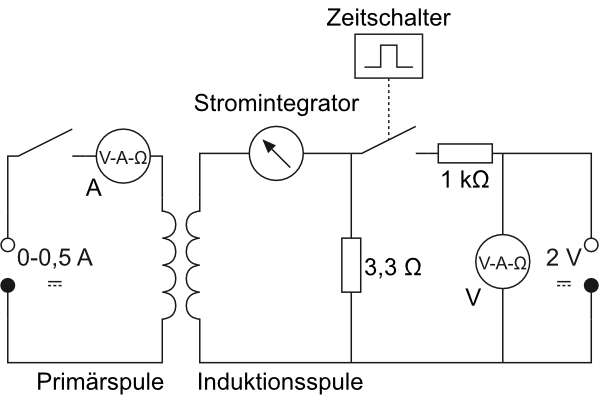
\includegraphics[scale=1.0]{IndSpuleAufbau.png}
	\caption{Magnetfeldmessung mit der Induktionsspule \cite[Datum: 09.10.2014]{LP13}}	 
	 \label{fig:IndSpule}
\end{figure}
Danach misst man das Magnetfeld der Langen Spule (Primärspule) mit der Induktionsspule nach dem Aufbau aus Abb. \ref{fig:IndSpule}, indem der Schalter im Primärkreis kurz geöffnet und wieder geschlossen wird.
Der durch den erzeugten Spannungspuls resultierende Strom wird über das Ladungsmessgerät integriert.
Für verschiedene Positionen auf der Spulenachse wird die Anzeige des Ladungsmessgerätes notiert.
Die Schrittweite beträgt dabei $2\,$cm und die Messung wird auch außerhalb der Spule fortgeführt.\\
Zu den weiteren Messungen wird die Hall-Sonde benutzt.
Diese schließt man an den Strom an und auf dem Display erscheint das gemessene Magnetfeld in Gauss.
Man startet bei allen drei Spulen (inkl. Helmholtzspule) in der Mitte der Spule und bewegt die Sonde bei jeder Messung um $1\,$cm heraus.
Zuletzt werden die Daten der einzelnen Spulen wie Länge, Durchmesser und Wicklungszahl notiert.


\section{Auswertung}
\label{sec:auswertung}
\subsection{Eichen des Stromintegrators}
Die verwendeten Widerstände waren:
\begin{itemize}
	\item $R_1=1\si{\kilo\ohm}$
	\item $R_2=3.3\si\ohm$
	\item Innenwiderstand des Stromintegrators $R_\text{int}$
	\item Spulenwiderstand $R_L$
\end{itemize}
Der Strom, der durch den Integrator fließt, wird mit $I_\kappa$ bezeichnet.
Aufgrund der Reihen- und Parallelschaltung der verschiedenen Widerstände ergibt sich ein Gesamtwiderstand von 
\begin{align}
		R_\text{ges}=R_1+\left(\frac{1}{R_2}+\frac{1}{R_L+R_\text{int}}\right)^{-1}\,.
\end{align}
Nach den Regeln für die Spannung an Parallelschaltungen gilt:
\begin{align*}
	R_2 I_2=(R_L+R_\text{int})I_\kappa\\
	\Rightarrow I_2=\frac{R_L+R_\text{int}}{R_2}I_\kappa\,.
\end{align*}
Damit kann der Gesamtstrom berechnet werden:
\begin{align*}
	I_\text{ges}&=I_\kappa+I_2=I_\kappa\left(1+\frac{R_L+R_\text{int}}{R_2}\right)\\
	\Rightarrow I_\kappa&=\frac{I_\text{ges}}{1+\frac{R_L+R_\text{int}}{R_2}}\,.
\end{align*}
Woraus sich der Widerstand der Spule und dem Integrator wie folgt ergibt:
\begin{align}
	R_\kappa=R_\text{int}+R_L=\frac U{I_\kappa}=\frac{U}{I_\text{ges}}\left(1+\frac{R_L+R_\text{int}}{R_2}\right)=R_\text{ges}\left(1+\frac{R_L+R_\text{int}}{R_2}\right)\,.
\end{align}
Der durch den Stromintegrator fließende Strom $I_\kappa$ bei einer anliegenden Spannung von $U_\text{int}$ beträgt
\begin{align}
	U_\text{int}&=\frac{U_\text{ges}R_\text{int}}{R_\text{int}+R_1}\\
	I_\kappa&=\frac{U_\text{int}}{R_\text{int}+R_L}\approx 6.85\cdot 10^{-7}\si\ampere\,.
\end{align}

Die Widerstände werden als fehlerfrei angenommen, da sie als Herstellerangaben im Vergleich zu den sonstigen auftretenden Fehlerquellen zu vernachlässigen sind.
Die Eichkonstante $\kappa$, welche das Verhältnis der angezeigten Skalenteilen zu den geflossenen Coulomb angibt, wurde mit der linearen Regression
\begin{align*}
	y=\kappa\cdot x
\end{align*}
bestimmt.
Es ergibt sich
\begin{align}
	\kappa=(426.9 \pm 0.4)\,\si{\pico\coulomb\per Skt.}\,.
\end{align}
Da der Fehler so gering ist, wird er in der folgenden Berechnung nicht berücksichtigt.
\begin{figure}[!htb]
	\centering
	% GNUPLOT: LaTeX picture with Postscript
\begingroup
  \makeatletter
  \providecommand\color[2][]{%
    \GenericError{(gnuplot) \space\space\space\@spaces}{%
      Package color not loaded in conjunction with
      terminal option `colourtext'%
    }{See the gnuplot documentation for explanation.%
    }{Either use 'blacktext' in gnuplot or load the package
      color.sty in LaTeX.}%
    \renewcommand\color[2][]{}%
  }%
  \providecommand\includegraphics[2][]{%
    \GenericError{(gnuplot) \space\space\space\@spaces}{%
      Package graphicx or graphics not loaded%
    }{See the gnuplot documentation for explanation.%
    }{The gnuplot epslatex terminal needs graphicx.sty or graphics.sty.}%
    \renewcommand\includegraphics[2][]{}%
  }%
  \providecommand\rotatebox[2]{#2}%
  \@ifundefined{ifGPcolor}{%
    \newif\ifGPcolor
    \GPcolortrue
  }{}%
  \@ifundefined{ifGPblacktext}{%
    \newif\ifGPblacktext
    \GPblacktexttrue
  }{}%
  % define a \g@addto@macro without @ in the name:
  \let\gplgaddtomacro\g@addto@macro
  % define empty templates for all commands taking text:
  \gdef\gplbacktext{}%
  \gdef\gplfronttext{}%
  \makeatother
  \ifGPblacktext
    % no textcolor at all
    \def\colorrgb#1{}%
    \def\colorgray#1{}%
  \else
    % gray or color?
    \ifGPcolor
      \def\colorrgb#1{\color[rgb]{#1}}%
      \def\colorgray#1{\color[gray]{#1}}%
      \expandafter\def\csname LTw\endcsname{\color{white}}%
      \expandafter\def\csname LTb\endcsname{\color{black}}%
      \expandafter\def\csname LTa\endcsname{\color{black}}%
      \expandafter\def\csname LT0\endcsname{\color[rgb]{1,0,0}}%
      \expandafter\def\csname LT1\endcsname{\color[rgb]{0,1,0}}%
      \expandafter\def\csname LT2\endcsname{\color[rgb]{0,0,1}}%
      \expandafter\def\csname LT3\endcsname{\color[rgb]{1,0,1}}%
      \expandafter\def\csname LT4\endcsname{\color[rgb]{0,1,1}}%
      \expandafter\def\csname LT5\endcsname{\color[rgb]{1,1,0}}%
      \expandafter\def\csname LT6\endcsname{\color[rgb]{0,0,0}}%
      \expandafter\def\csname LT7\endcsname{\color[rgb]{1,0.3,0}}%
      \expandafter\def\csname LT8\endcsname{\color[rgb]{0.5,0.5,0.5}}%
    \else
      % gray
      \def\colorrgb#1{\color{black}}%
      \def\colorgray#1{\color[gray]{#1}}%
      \expandafter\def\csname LTw\endcsname{\color{white}}%
      \expandafter\def\csname LTb\endcsname{\color{black}}%
      \expandafter\def\csname LTa\endcsname{\color{black}}%
      \expandafter\def\csname LT0\endcsname{\color{black}}%
      \expandafter\def\csname LT1\endcsname{\color{black}}%
      \expandafter\def\csname LT2\endcsname{\color{black}}%
      \expandafter\def\csname LT3\endcsname{\color{black}}%
      \expandafter\def\csname LT4\endcsname{\color{black}}%
      \expandafter\def\csname LT5\endcsname{\color{black}}%
      \expandafter\def\csname LT6\endcsname{\color{black}}%
      \expandafter\def\csname LT7\endcsname{\color{black}}%
      \expandafter\def\csname LT8\endcsname{\color{black}}%
    \fi
  \fi
  \setlength{\unitlength}{0.0500bp}%
  \begin{picture}(7200.00,5040.00)%
    \gplgaddtomacro\gplbacktext{%
      \csname LTb\endcsname%
      \put(1254,704){\makebox(0,0)[r]{\strut{} 0}}%
      \put(1254,1074){\makebox(0,0)[r]{\strut{} 0.1}}%
      \put(1254,1444){\makebox(0,0)[r]{\strut{} 0.2}}%
      \put(1254,1815){\makebox(0,0)[r]{\strut{} 0.3}}%
      \put(1254,2185){\makebox(0,0)[r]{\strut{} 0.4}}%
      \put(1254,2555){\makebox(0,0)[r]{\strut{} 0.5}}%
      \put(1254,2925){\makebox(0,0)[r]{\strut{} 0.6}}%
      \put(1254,3295){\makebox(0,0)[r]{\strut{} 0.7}}%
      \put(1254,3665){\makebox(0,0)[r]{\strut{} 0.8}}%
      \put(1254,4036){\makebox(0,0)[r]{\strut{} 0.9}}%
      \put(1254,4406){\makebox(0,0)[r]{\strut{} 1}}%
      \put(1254,4776){\makebox(0,0)[r]{\strut{} 1.1}}%
      \put(1386,484){\makebox(0,0){\strut{} 0}}%
      \put(2005,484){\makebox(0,0){\strut{} 100}}%
      \put(2624,484){\makebox(0,0){\strut{} 200}}%
      \put(3243,484){\makebox(0,0){\strut{} 300}}%
      \put(3862,484){\makebox(0,0){\strut{} 400}}%
      \put(4482,484){\makebox(0,0){\strut{} 500}}%
      \put(5101,484){\makebox(0,0){\strut{} 600}}%
      \put(5720,484){\makebox(0,0){\strut{} 700}}%
      \put(6339,484){\makebox(0,0){\strut{} 800}}%
      \put(6958,484){\makebox(0,0){\strut{} 900}}%
      \put(484,2740){\rotatebox{90}{\makebox(0,0){\strut{}Ladung [mC]}}}%
      \put(4172,154){\makebox(0,0){\strut{}Skalen-Teile}}%
    }%
    \gplgaddtomacro\gplfronttext{%
      \csname LTb\endcsname%
      \put(3762,4603){\makebox(0,0)[r]{\strut{}Messwerte}}%
      \csname LTb\endcsname%
      \put(3762,4383){\makebox(0,0)[r]{\strut{}Regressionsgerade}}%
    }%
    \gplbacktext
    \put(0,0){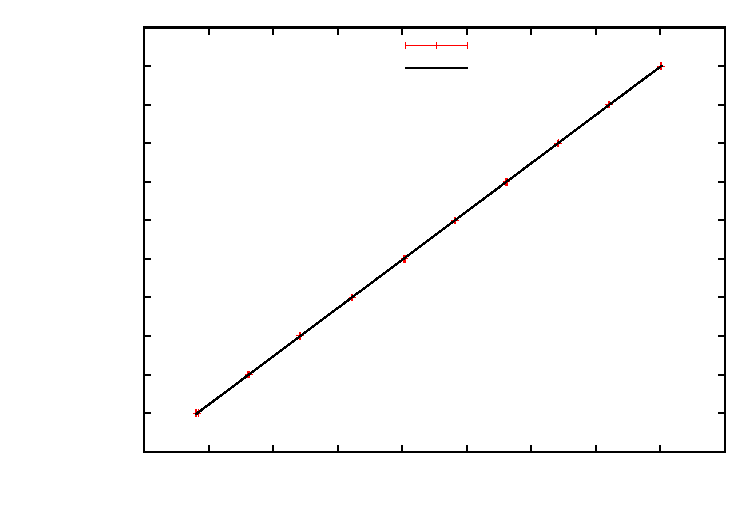
\includegraphics{Eichen}}%
    \gplfronttext
  \end{picture}%
\endgroup

	\caption{Ladung in Abhängigkeit der angezeigten Skalenteile.}
	\label{fig:Eichen}
\end{figure}

\subsection{Vergleich der beiden Messmethoden}
In Abbildung \ref{fig:LangIndHall} sind die Messwerte der beiden Messmethoden sowie der theoretische Verlauf des Magnetfeldes an der langen Spule aufgetragen.
Hierbei fällt auf, dass die Messung der Hallsonde innerhalb der Spule stärker von der Theorie abweicht, als die der Induktionsspule.
\begin{figure}[!htb]
	\centering
	% GNUPLOT: LaTeX picture with Postscript
\begingroup
  \makeatletter
  \providecommand\color[2][]{%
    \GenericError{(gnuplot) \space\space\space\@spaces}{%
      Package color not loaded in conjunction with
      terminal option `colourtext'%
    }{See the gnuplot documentation for explanation.%
    }{Either use 'blacktext' in gnuplot or load the package
      color.sty in LaTeX.}%
    \renewcommand\color[2][]{}%
  }%
  \providecommand\includegraphics[2][]{%
    \GenericError{(gnuplot) \space\space\space\@spaces}{%
      Package graphicx or graphics not loaded%
    }{See the gnuplot documentation for explanation.%
    }{The gnuplot epslatex terminal needs graphicx.sty or graphics.sty.}%
    \renewcommand\includegraphics[2][]{}%
  }%
  \providecommand\rotatebox[2]{#2}%
  \@ifundefined{ifGPcolor}{%
    \newif\ifGPcolor
    \GPcolortrue
  }{}%
  \@ifundefined{ifGPblacktext}{%
    \newif\ifGPblacktext
    \GPblacktexttrue
  }{}%
  % define a \g@addto@macro without @ in the name:
  \let\gplgaddtomacro\g@addto@macro
  % define empty templates for all commands taking text:
  \gdef\gplbacktext{}%
  \gdef\gplfronttext{}%
  \makeatother
  \ifGPblacktext
    % no textcolor at all
    \def\colorrgb#1{}%
    \def\colorgray#1{}%
  \else
    % gray or color?
    \ifGPcolor
      \def\colorrgb#1{\color[rgb]{#1}}%
      \def\colorgray#1{\color[gray]{#1}}%
      \expandafter\def\csname LTw\endcsname{\color{white}}%
      \expandafter\def\csname LTb\endcsname{\color{black}}%
      \expandafter\def\csname LTa\endcsname{\color{black}}%
      \expandafter\def\csname LT0\endcsname{\color[rgb]{1,0,0}}%
      \expandafter\def\csname LT1\endcsname{\color[rgb]{0,1,0}}%
      \expandafter\def\csname LT2\endcsname{\color[rgb]{0,0,1}}%
      \expandafter\def\csname LT3\endcsname{\color[rgb]{1,0,1}}%
      \expandafter\def\csname LT4\endcsname{\color[rgb]{0,1,1}}%
      \expandafter\def\csname LT5\endcsname{\color[rgb]{1,1,0}}%
      \expandafter\def\csname LT6\endcsname{\color[rgb]{0,0,0}}%
      \expandafter\def\csname LT7\endcsname{\color[rgb]{1,0.3,0}}%
      \expandafter\def\csname LT8\endcsname{\color[rgb]{0.5,0.5,0.5}}%
    \else
      % gray
      \def\colorrgb#1{\color{black}}%
      \def\colorgray#1{\color[gray]{#1}}%
      \expandafter\def\csname LTw\endcsname{\color{white}}%
      \expandafter\def\csname LTb\endcsname{\color{black}}%
      \expandafter\def\csname LTa\endcsname{\color{black}}%
      \expandafter\def\csname LT0\endcsname{\color{black}}%
      \expandafter\def\csname LT1\endcsname{\color{black}}%
      \expandafter\def\csname LT2\endcsname{\color{black}}%
      \expandafter\def\csname LT3\endcsname{\color{black}}%
      \expandafter\def\csname LT4\endcsname{\color{black}}%
      \expandafter\def\csname LT5\endcsname{\color{black}}%
      \expandafter\def\csname LT6\endcsname{\color{black}}%
      \expandafter\def\csname LT7\endcsname{\color{black}}%
      \expandafter\def\csname LT8\endcsname{\color{black}}%
    \fi
  \fi
  \setlength{\unitlength}{0.0500bp}%
  \begin{picture}(7200.00,5040.00)%
    \gplgaddtomacro\gplbacktext{%
      \csname LTb\endcsname%
      \put(814,1804){\makebox(0,0)[r]{\strut{} 0}}%
      \put(814,2228){\makebox(0,0)[r]{\strut{} 2}}%
      \put(814,2653){\makebox(0,0)[r]{\strut{} 4}}%
      \put(814,3077){\makebox(0,0)[r]{\strut{} 6}}%
      \put(814,3502){\makebox(0,0)[r]{\strut{} 8}}%
      \put(814,3926){\makebox(0,0)[r]{\strut{} 10}}%
      \put(814,4351){\makebox(0,0)[r]{\strut{} 12}}%
      \put(814,4775){\makebox(0,0)[r]{\strut{} 14}}%
      \put(946,1584){\makebox(0,0){\strut{}-20}}%
      \put(1783,1584){\makebox(0,0){\strut{}-10}}%
      \put(2619,1584){\makebox(0,0){\strut{} 0}}%
      \put(3456,1584){\makebox(0,0){\strut{} 10}}%
      \put(4293,1584){\makebox(0,0){\strut{} 20}}%
      \put(5130,1584){\makebox(0,0){\strut{} 30}}%
      \put(5966,1584){\makebox(0,0){\strut{} 40}}%
      \put(6803,1584){\makebox(0,0){\strut{} 50}}%
      \put(176,3289){\rotatebox{-270}{\makebox(0,0){\strut{}Magnetfeld [Gs]}}}%
      \put(3874,1254){\makebox(0,0){\strut{}Position [cm]}}%
    }%
    \gplgaddtomacro\gplfronttext{%
      \csname LTb\endcsname%
      \put(4833,833){\makebox(0,0)[r]{\strut{}Induktion}}%
      \csname LTb\endcsname%
      \put(4833,613){\makebox(0,0)[r]{\strut{}Hallsonde}}%
      \csname LTb\endcsname%
      \put(4833,393){\makebox(0,0)[r]{\strut{}Näherung lange Spule}}%
      \csname LTb\endcsname%
      \put(4833,173){\makebox(0,0)[r]{\strut{}theoretischer Verlauf}}%
    }%
    \gplbacktext
    \put(0,0){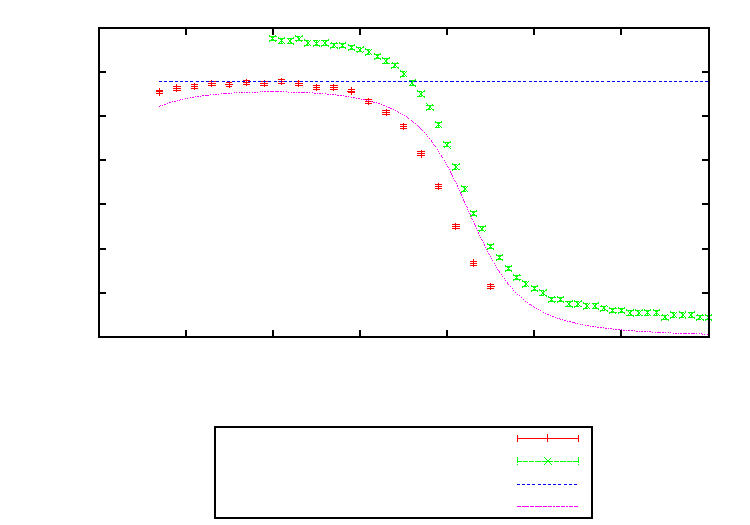
\includegraphics{LangIndHall}}%
    \gplfronttext
  \end{picture}%
\endgroup

	\caption{Verlauf des Magnetfeldes: Vergleich der beiden Messmethoden mit der Theorie anhand der Langen Spule.}
	\label{fig:LangIndHall}
\end{figure}
\subsection{Messung mit der Hallsonde}
In Diagramm \ref{fig:HallVergleich} sind die Messwerte der Hallsonde für die lange und die dicke Spule mit den theoretischen Messwerten aufgetragen.
Die Näherung der Langen Spule ist, wie deutlich zu erkennen, nur im Inneren der Spule halbwegs akkurat.
Sie entspricht natürlich für die lange Spule eher der Realität und erstaunlicherweise genauer den Messwerten bis ca. 15cm von der Mitte entfernt.

\begin{figure}[!htb]
	\centering
	% GNUPLOT: LaTeX picture with Postscript
\begingroup
  \makeatletter
  \providecommand\color[2][]{%
    \GenericError{(gnuplot) \space\space\space\@spaces}{%
      Package color not loaded in conjunction with
      terminal option `colourtext'%
    }{See the gnuplot documentation for explanation.%
    }{Either use 'blacktext' in gnuplot or load the package
      color.sty in LaTeX.}%
    \renewcommand\color[2][]{}%
  }%
  \providecommand\includegraphics[2][]{%
    \GenericError{(gnuplot) \space\space\space\@spaces}{%
      Package graphicx or graphics not loaded%
    }{See the gnuplot documentation for explanation.%
    }{The gnuplot epslatex terminal needs graphicx.sty or graphics.sty.}%
    \renewcommand\includegraphics[2][]{}%
  }%
  \providecommand\rotatebox[2]{#2}%
  \@ifundefined{ifGPcolor}{%
    \newif\ifGPcolor
    \GPcolortrue
  }{}%
  \@ifundefined{ifGPblacktext}{%
    \newif\ifGPblacktext
    \GPblacktexttrue
  }{}%
  % define a \g@addto@macro without @ in the name:
  \let\gplgaddtomacro\g@addto@macro
  % define empty templates for all commands taking text:
  \gdef\gplbacktext{}%
  \gdef\gplfronttext{}%
  \makeatother
  \ifGPblacktext
    % no textcolor at all
    \def\colorrgb#1{}%
    \def\colorgray#1{}%
  \else
    % gray or color?
    \ifGPcolor
      \def\colorrgb#1{\color[rgb]{#1}}%
      \def\colorgray#1{\color[gray]{#1}}%
      \expandafter\def\csname LTw\endcsname{\color{white}}%
      \expandafter\def\csname LTb\endcsname{\color{black}}%
      \expandafter\def\csname LTa\endcsname{\color{black}}%
      \expandafter\def\csname LT0\endcsname{\color[rgb]{1,0,0}}%
      \expandafter\def\csname LT1\endcsname{\color[rgb]{0,1,0}}%
      \expandafter\def\csname LT2\endcsname{\color[rgb]{0,0,1}}%
      \expandafter\def\csname LT3\endcsname{\color[rgb]{1,0,1}}%
      \expandafter\def\csname LT4\endcsname{\color[rgb]{0,1,1}}%
      \expandafter\def\csname LT5\endcsname{\color[rgb]{1,1,0}}%
      \expandafter\def\csname LT6\endcsname{\color[rgb]{0,0,0}}%
      \expandafter\def\csname LT7\endcsname{\color[rgb]{1,0.3,0}}%
      \expandafter\def\csname LT8\endcsname{\color[rgb]{0.5,0.5,0.5}}%
    \else
      % gray
      \def\colorrgb#1{\color{black}}%
      \def\colorgray#1{\color[gray]{#1}}%
      \expandafter\def\csname LTw\endcsname{\color{white}}%
      \expandafter\def\csname LTb\endcsname{\color{black}}%
      \expandafter\def\csname LTa\endcsname{\color{black}}%
      \expandafter\def\csname LT0\endcsname{\color{black}}%
      \expandafter\def\csname LT1\endcsname{\color{black}}%
      \expandafter\def\csname LT2\endcsname{\color{black}}%
      \expandafter\def\csname LT3\endcsname{\color{black}}%
      \expandafter\def\csname LT4\endcsname{\color{black}}%
      \expandafter\def\csname LT5\endcsname{\color{black}}%
      \expandafter\def\csname LT6\endcsname{\color{black}}%
      \expandafter\def\csname LT7\endcsname{\color{black}}%
      \expandafter\def\csname LT8\endcsname{\color{black}}%
    \fi
  \fi
  \setlength{\unitlength}{0.0500bp}%
  \begin{picture}(7200.00,5040.00)%
    \gplgaddtomacro\gplbacktext{%
      \csname LTb\endcsname%
      \put(814,2244){\makebox(0,0)[r]{\strut{}-2}}%
      \put(814,2560){\makebox(0,0)[r]{\strut{} 0}}%
      \put(814,2877){\makebox(0,0)[r]{\strut{} 2}}%
      \put(814,3193){\makebox(0,0)[r]{\strut{} 4}}%
      \put(814,3510){\makebox(0,0)[r]{\strut{} 6}}%
      \put(814,3826){\makebox(0,0)[r]{\strut{} 8}}%
      \put(814,4142){\makebox(0,0)[r]{\strut{} 10}}%
      \put(814,4459){\makebox(0,0)[r]{\strut{} 12}}%
      \put(814,4775){\makebox(0,0)[r]{\strut{} 14}}%
      \put(946,2024){\makebox(0,0){\strut{} 0}}%
      \put(2117,2024){\makebox(0,0){\strut{} 10}}%
      \put(3289,2024){\makebox(0,0){\strut{} 20}}%
      \put(4460,2024){\makebox(0,0){\strut{} 30}}%
      \put(5632,2024){\makebox(0,0){\strut{} 40}}%
      \put(6803,2024){\makebox(0,0){\strut{} 50}}%
      \put(176,3509){\rotatebox{-270}{\makebox(0,0){\strut{}Magnetfeld [Gs]}}}%
      \put(3874,1694){\makebox(0,0){\strut{}Position [cm]}}%
    }%
    \gplgaddtomacro\gplfronttext{%
      \csname LTb\endcsname%
      \put(5691,1273){\makebox(0,0)[r]{\strut{}Lange Spule}}%
      \csname LTb\endcsname%
      \put(5691,1053){\makebox(0,0)[r]{\strut{}Lange Spule: Näherung lange Spule}}%
      \csname LTb\endcsname%
      \put(5691,833){\makebox(0,0)[r]{\strut{}Lange Spule: theoretischer Verlauf}}%
      \csname LTb\endcsname%
      \put(5691,613){\makebox(0,0)[r]{\strut{}Dicke Spule}}%
      \csname LTb\endcsname%
      \put(5691,393){\makebox(0,0)[r]{\strut{}Dicke Spule: Näherung lange Spule}}%
      \csname LTb\endcsname%
      \put(5691,173){\makebox(0,0)[r]{\strut{}Dicke Spule: theoretischer Verlauf}}%
    }%
    \gplbacktext
    \put(0,0){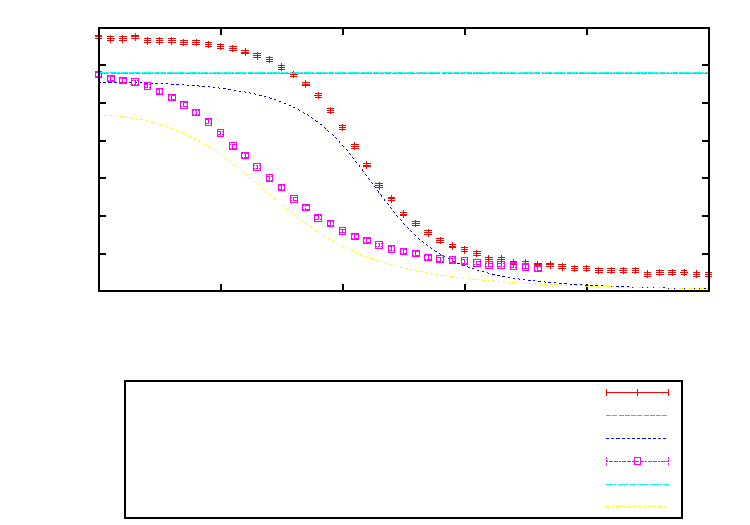
\includegraphics{Hall}}%
    \gplfronttext
  \end{picture}%
\endgroup

	\caption{Verlauf des Magnetfeldes: Vergleich der langen und der dicken Spule sowie jeweils mit der Theorie.}
	\label{fig:HallVergleich}
\end{figure}
\subsection{Homogenität der Magnetfelder}
In Abbildung \ref{fig:Homogen} sind die Messwerte der Hallsonde für alle Spulen aufgetragen.
Die Werte, welche nicht aufgenommen wurden, wurden um den jeweiligen Mittelpunkt der Spulen gespiegelt, da diese einen symmetrischen Verlauf besitzen.
Hierbei fällt auf, dass die Helmholtzspulen zwar außerhalb der Spulen einen sehr starken Abfall der Feldstärke besitzen, im Inneren ist ihr Magnetfeld jedoch deutlich homogener, als das der Dicken Spule.
Bei dieser fällt es zwar zum Rand hin nicht so schnell ab, es ist jedoch an keiner Stelle konstant.

In unserem Aufbau haben wir die Helmholtzspulen parallel angeschlossen, so dass nur der halbe Strom durch die einzelne Spule fließt.
Dies muss man in der Auswertung berücksichtigen, da sonst die Magnetfelder die doppelte Stärke hätten.

\begin{figure}[!htb]
	\centering
	% GNUPLOT: LaTeX picture with Postscript
\begingroup
  \makeatletter
  \providecommand\color[2][]{%
    \GenericError{(gnuplot) \space\space\space\@spaces}{%
      Package color not loaded in conjunction with
      terminal option `colourtext'%
    }{See the gnuplot documentation for explanation.%
    }{Either use 'blacktext' in gnuplot or load the package
      color.sty in LaTeX.}%
    \renewcommand\color[2][]{}%
  }%
  \providecommand\includegraphics[2][]{%
    \GenericError{(gnuplot) \space\space\space\@spaces}{%
      Package graphicx or graphics not loaded%
    }{See the gnuplot documentation for explanation.%
    }{The gnuplot epslatex terminal needs graphicx.sty or graphics.sty.}%
    \renewcommand\includegraphics[2][]{}%
  }%
  \providecommand\rotatebox[2]{#2}%
  \@ifundefined{ifGPcolor}{%
    \newif\ifGPcolor
    \GPcolortrue
  }{}%
  \@ifundefined{ifGPblacktext}{%
    \newif\ifGPblacktext
    \GPblacktexttrue
  }{}%
  % define a \g@addto@macro without @ in the name:
  \let\gplgaddtomacro\g@addto@macro
  % define empty templates for all commands taking text:
  \gdef\gplbacktext{}%
  \gdef\gplfronttext{}%
  \makeatother
  \ifGPblacktext
    % no textcolor at all
    \def\colorrgb#1{}%
    \def\colorgray#1{}%
  \else
    % gray or color?
    \ifGPcolor
      \def\colorrgb#1{\color[rgb]{#1}}%
      \def\colorgray#1{\color[gray]{#1}}%
      \expandafter\def\csname LTw\endcsname{\color{white}}%
      \expandafter\def\csname LTb\endcsname{\color{black}}%
      \expandafter\def\csname LTa\endcsname{\color{black}}%
      \expandafter\def\csname LT0\endcsname{\color[rgb]{1,0,0}}%
      \expandafter\def\csname LT1\endcsname{\color[rgb]{0,1,0}}%
      \expandafter\def\csname LT2\endcsname{\color[rgb]{0,0,1}}%
      \expandafter\def\csname LT3\endcsname{\color[rgb]{1,0,1}}%
      \expandafter\def\csname LT4\endcsname{\color[rgb]{0,1,1}}%
      \expandafter\def\csname LT5\endcsname{\color[rgb]{1,1,0}}%
      \expandafter\def\csname LT6\endcsname{\color[rgb]{0,0,0}}%
      \expandafter\def\csname LT7\endcsname{\color[rgb]{1,0.3,0}}%
      \expandafter\def\csname LT8\endcsname{\color[rgb]{0.5,0.5,0.5}}%
    \else
      % gray
      \def\colorrgb#1{\color{black}}%
      \def\colorgray#1{\color[gray]{#1}}%
      \expandafter\def\csname LTw\endcsname{\color{white}}%
      \expandafter\def\csname LTb\endcsname{\color{black}}%
      \expandafter\def\csname LTa\endcsname{\color{black}}%
      \expandafter\def\csname LT0\endcsname{\color{black}}%
      \expandafter\def\csname LT1\endcsname{\color{black}}%
      \expandafter\def\csname LT2\endcsname{\color{black}}%
      \expandafter\def\csname LT3\endcsname{\color{black}}%
      \expandafter\def\csname LT4\endcsname{\color{black}}%
      \expandafter\def\csname LT5\endcsname{\color{black}}%
      \expandafter\def\csname LT6\endcsname{\color{black}}%
      \expandafter\def\csname LT7\endcsname{\color{black}}%
      \expandafter\def\csname LT8\endcsname{\color{black}}%
    \fi
  \fi
  \setlength{\unitlength}{0.0500bp}%
  \begin{picture}(7200.00,5040.00)%
    \gplgaddtomacro\gplbacktext{%
      \csname LTb\endcsname%
      \put(814,1804){\makebox(0,0)[r]{\strut{}-5}}%
      \put(814,2299){\makebox(0,0)[r]{\strut{} 0}}%
      \put(814,2794){\makebox(0,0)[r]{\strut{} 5}}%
      \put(814,3290){\makebox(0,0)[r]{\strut{} 10}}%
      \put(814,3785){\makebox(0,0)[r]{\strut{} 15}}%
      \put(814,4280){\makebox(0,0)[r]{\strut{} 20}}%
      \put(814,4775){\makebox(0,0)[r]{\strut{} 25}}%
      \put(946,1584){\makebox(0,0){\strut{}-60}}%
      \put(1922,1584){\makebox(0,0){\strut{}-40}}%
      \put(2898,1584){\makebox(0,0){\strut{}-20}}%
      \put(3875,1584){\makebox(0,0){\strut{} 0}}%
      \put(4851,1584){\makebox(0,0){\strut{} 20}}%
      \put(5827,1584){\makebox(0,0){\strut{} 40}}%
      \put(6803,1584){\makebox(0,0){\strut{} 60}}%
      \put(176,3289){\rotatebox{-270}{\makebox(0,0){\strut{}Magnetfeld [Gs]}}}%
      \put(3874,1254){\makebox(0,0){\strut{}Position [cm]}}%
    }%
    \gplgaddtomacro\gplfronttext{%
      \csname LTb\endcsname%
      \put(5097,833){\makebox(0,0)[r]{\strut{}Lange Spule}}%
      \csname LTb\endcsname%
      \put(5097,613){\makebox(0,0)[r]{\strut{}Dicke Spule}}%
      \csname LTb\endcsname%
      \put(5097,393){\makebox(0,0)[r]{\strut{}Helmholtzspule}}%
      \csname LTb\endcsname%
      \put(5097,173){\makebox(0,0)[r]{\strut{}theo. Max. Helmholtzspule}}%
    }%
    \gplbacktext
    \put(0,0){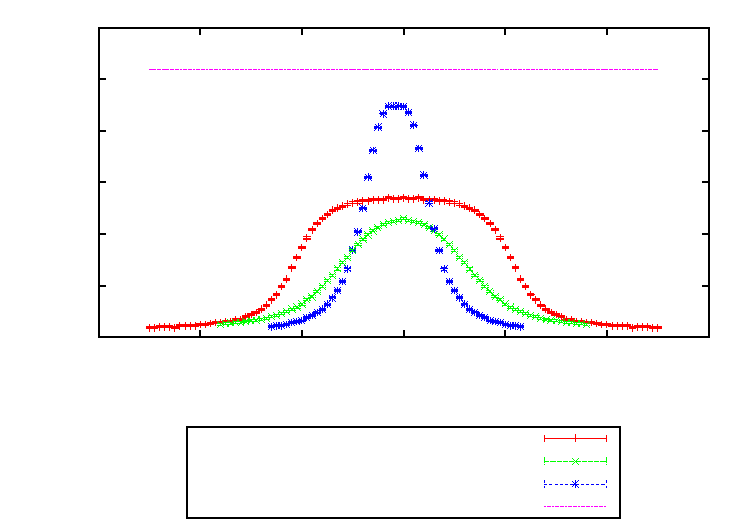
\includegraphics{Homogen}}%
    \gplfronttext
  \end{picture}%
\endgroup

	\caption{Verlauf des Magnetfeldes der 3 Spulen: Messung mit der Hallsonde.}
	\label{fig:Homogen}
\end{figure}

\subsection{Bestimmung von $\mu_0$}
In Tabelle \ref{tab:mu} sind die berechneten $\mu_0$ zu sehen, welche nach der Formel
\begin{align*}
	B=\mu_0 H
\end{align*}
bestimmt werden.
Dabei werden für das $B$-Feld die Messwerte und für das $H$-Feld die theoretisch nach Formeln \eqref{eq:BSpule} und \eqref{eq:BHelm} bestimmten Werte.
Dies haben wir über das Fitten der Theoriekurve an die Messwerte über den Faktor $\mu_0$ durchgeführt, da so gleich die gewichteten Mittelwerte der jeweiligen Kurven ermittelt werden.
Zu beachten ist hierbei, dass es sich bei den Näherungen des theoretischen $B$-Feldes um Taylor-Entwicklungen um die Mitte der Spule handelt, welche außerhalb der Spulen deutlich ungenauer werden.

\begin{table}[!htb]
	\centering
	\begin{tabular}{|c|c|c|}
	\hline
	Messungmethode & Spule & $\mu_0$ [$10^{-7}\,\si{\henry\per\meter}$]\\
	\hline
	\hline
	Induktionsspule & Lange Spule & $13.020 \pm 0.020$\\
	\hline
	          & Lange Spule & $13.67 \pm 0.11$ \\
	Hallsonde & Dicke Spule & $13.28 \pm 0.13$ \\
	          & Helmholtzspule & $12.39 \pm 0.05$ \\
	\hline\hline
	Gew. Mittelwert	& & $13.308\pm 0.006$ \\\hline
	\end{tabular}
	\caption{Aus den verschiedenen Messungen bestimmte magnetische Feldkonstante}
	\label{tab:mu}
\end{table}


\section{Diskussion}
\label{sec:diskussion}
\subsection{Eichen des Stromintegrators}
In der Graphik \ref{fig:Eichen} sind die Ladungen gegen die vom Stromintegrator angezeigten Skalenteile aufgetragen.
Die Messwerte liegen sehr gut auf einer Geraden, so dass sich nur eine Unsicherheit der Geradensteigung (der Eichkonstante) $\kappa$ von $0.1\%$ ergibt.
Dies spricht für die Qualität des  Integrators, da er selbst bei einer halben Sekunde immer noch keine Sättigung zeigt.
Darauf müsste man bei anderen Versuchsaufbauten gegebenenfalls achten und den Widerstand $R_2$ dementsprechend anpassen.

\subsection{Vergleich der Messmethoden}
In Abb. \ref{fig:LangIndHall} sind die Messwerte der beiden Methoden eingezeichnet, sowie die theoretische Kurve.
Dabei fällt auf, dass beide Messwerte innerhalb der Spule über dem theoretischen Wert liegen.
Die Messung der Induktionsspule ist jedoch dichter an diesem.
Die Induktionsspule ist jedoch im Bereich von 15cm bis zu der letzten Messung fast identisch mit der Theoriekurve.

\subsection{Hallsonde}
In dem Diagramm \ref{fig:HallVergleich} sind die Messwerte der Hallsonde zusammen mit den Theoriekurven für die dicke und die lange Spule aufgetragen.
Bei beiden liegen die Messungen im Inneren der Spulen über den berechneten Werten und fallen danach darunter.
Die Messwerte beinhalten zwar kaum die erwarteten in ihren Fehlerintervallen, jedoch folgen sie deutlich den Kurven, so dass sich vermuten lässt, dass im Inneren Effekte vernachlässigt wurden, welche die Werte beeinflussten.
Auch kann man gut sehen, dass die Felder im Inneren nicht so groß werden, wie unter der Näherung der langen Spule.


\subsection{Homogenität der Magnetfelder}
In Abbildung \ref{fig:Homogen} sind die Messwerte der Hallsonde für alle Spulen aufgetragen.
Die Werte, welche nicht aufgenommen wurden, wurden um den Mittelpunkt der Spule gespiegelt, da diese einen symmetrischen Verlauf besitzt.
Wie zu erwarten, hat die dicke Spule keinen nennenswerten Bereich, in dem sie ein homogenes Magnetfeld besitzt, während die Helmholzspulen auf 10cm eine annähernd konstante Feldstärke aufweisen.
Die lange Spule ist natürlich auf einem noch größeren Bereich (ca. 30cm) in guter Näherung mit einem homogenen Feld gefüllt.

Wir haben die Helmholtzspulen parallel und nicht in Reihe geschaltet, wie es eigentlich vorgesehen ist.
Dies hat den Nachteil, dass so der Strom in den Spulen nicht gleich groß ist, falls sie unterschiedliche Widerstände haben, so dass das Magnetfeld nicht homogen ist.
In unserem Fall war dies augenscheinlich nicht besonders stark der Fall, für zukünftige Versuche sollte man aber darauf achten, dies zu vermeiden.

\subsection{Bestimmung von $\mu_0$}
Der gewichtete Mittelwert aller bestimmten $\mu_0$ aus Tabelle \ref{tab:mu} beträgt  $(13.308\pm 0.006)\cdot 10^{-7}\si{\newton\ampere^{-2}}$, was um ungefähr 6\% größer ist, als der tatsächliche Wert von $4\pi\cdot10^{-7}\si{\newton\ampere^{-2}}$.
Dieser liegt nicht im Fehlerintervall, was vermutlich an der zu geringen Fehlerabschätzung und der Vernachlässigung einiger Fehler liegt.

\bibliography{literatur}
\bibliographystyle{babalpha}
\end{document}
